\documentclass[10pt]{article}

\usepackage{akteach}
\usepackage{amsmath}
\usepackage{amsfonts}
\usepackage{amssymb}
\usepackage{amsthm}
\usepackage{float}
\usepackage{algpseudocode}
\usepackage[all]{xy}


\newcommand{\C}{\mathbb{C}}
\newcommand{\Q}{\mathbb{Q}}
\newcommand{\K}{\mathbb{K}}
\newcommand{\proj}{\mathbb{P}}
\newcommand{\T}{\mathbb{T}}
\newcommand{\F}{\mathbb{F}}
\newcommand{\Z}{\mathbb{Z}}
\newcommand{\N}{\mathbb{N}}
\newcommand{\cp}{\mathbb{C}P}
\newcommand{\A}{\mathcal{A}}
\newcommand{\BB}{\mathcal{B}}
\newcommand{\CC}{\mathcal{C}}
\newcommand{\NN}{\mathcal{N}}
\newcommand{\MM}{\mathcal{M}}
\newcommand{\E}{\mathcal{E}}
\newcommand{\FF}{\mathcal{F}}
\newcommand{\G}{\mathcal{G}}
\newcommand{\eps}{\varepsilon}
\newcommand{\Hom}{\text{Hom}}
\newcommand{\Div}{\text{div}}
\newcommand{\Res}{\text{Res}}
\newcommand{\ord}{\text{ord}}
\newcommand{\Deg}{\text{deg}}
\newcommand{\mult}{\text{mult}}

\newcommand{\id}{\text{id}}
\newcommand{\Tr}{\text{Tr}}
\newcommand{\ad}{\text{ad}}
\newcommand{\Ad}{\text{Ad}}
\newcommand{\Aut}{\text{Aut}}
\newcommand{\der}{\text{der}}
\newcommand{\GL}{\text{GL}}
\newcommand{\gl}{\mathfrak{gl}}
\newcommand{\rad}{\mathfrak{rad}}
\newcommand{\inhook}{\hookrightarrow}

\begin{document}

\akteachheader{Numerical Analysis (CS 450)}%
{Homework Set 1, Bill Karr}

\akteachprobhead{%
  Problem 1: Develop the Cholesky factorization (15 points)
}

\begin{enumerate}[(a)]

\item[(b)] Given a SPD matrix $A$, we can write $ A = L L^T $ where $L$ is a lower triangular matrix with positive diagonal entries. If $$A = \begin{bmatrix}
a_{11} & a_{21}  & a_{31} \\
a_{21} & a_{22} & a_{32} \\
a_{31} & a_{32} & a_{33}
\end{bmatrix}, \quad
L = \begin{bmatrix}
l_{11} & 0  & 0 \\
l_{21} & l_{22} & 0 \\
l_{31} & l_{32} & l_{33}
\end{bmatrix},
$$ and $$
A = L L^T = \begin{bmatrix}
l_{11} & 0  & 0 \\
l_{21} & l_{22} & 0 \\
l_{31} & l_{32} & l_{33}
\end{bmatrix} \begin{bmatrix}
l_{11} & l_{21} & l_{31} \\
0 & l_{22} & l_{32} \\
0 & 0 & l_{33}
\end{bmatrix} = \begin{bmatrix}
l_{11}^2 & l_{11} l_{21} & l_{11} l_{31} \\
l_{11} l_{21} & l_{21}^2 + l_{22}^2 & l_{21} l_{31} + l_{22} l_{32} \\
l_{11} l_{31}  & l_{21} l_{31} + l_{22} l_{32} & l_{31}^2 + l_{32}^2 + l_{33}^2
\end{bmatrix}.
$$ We can solve for all of the entries of $L$ by solving successively for each row. \begin{align*}
l_{11} &= \sqrt{a_{11}} &  & \\
l_{21} &= \frac{a_{21}}{l_{11}}  & l_{22} &= \sqrt{a_{22} - l_{21}^2} & \\
l_{31} &= \frac{a_{31}}{l_{11}} & l_{32} &= \frac{a_{32} - l_{21} l_{31} }{l_{22}} & l_{33} = \sqrt{a_{33} - l_{31}^2 - l_{32}^2 }
\end{align*} We can solve each row using the previous one and obtain each entry of $L$ in terms of the $ a_{ij} $. 

\item[(c)] We can generalize this process to when $A$ is $n \times n$ with an algorithm using the following pseudocode. 

\begin{algorithmic}
\For {$i = 1 : n$}
    \For {$j = 1: i - 1$}
     $ L_{ij} = \frac{A_{ij} - \sum_{k = 1}^{j - 1} L_{ik} L_{jk}}{L_{jj}} $
    \EndFor \\
$L_{ii} = \sqrt{ A_{ii} - \sum_{k = 1}^{i - 1} L_{ik} L_{ik}  } $
\EndFor
\end{algorithmic}

\item[(d)] See \verb+cs450hw2p1.py+ for code. My results were:

\begin{verbatim}
We compute 3 random 20x20 SPD matrices, compute their
Cholesky factors, measure the relative error between LL.T and A, and print
the condition number of A.

For matrix 1 :
relative error = 9.8432266534e-17
cond(A) = 84677.106702

For matrix 2 :
relative error = 1.0513418823e-16
cond(A) = 8543.8395193

For matrix 3 :
relative error = 9.80546815682e-17
cond(A) = 7189520.36827
\end{verbatim}

\item[(e)] See \verb+cs450hw2p1.py+ for code. My results were:

\begin{verbatim}
We compute random SPD matrices A of size 5x5, 10x10, and
100x100, compute their Cholesky factors L, and then compute the determinant
of A by computing the determinant of L and squaring it, and the relative
error between this value and numpy's determinant of A.

n = 5
numpy det(A) = 0.000177716168912
det(L)^2 = 0.000177716168912
relative error = 7.21413857169e-14

n = 10
numpy det(A) = 7.75296542487e-05
det(L)^2 = 7.75296542487e-05
relative error = 2.53466426063e-14

n = 100
numpy det(A) = 3.97219657038e+51
det(L)^2 = 3.97219657042e+51
relative error = 9.72292869882e-12

\end{verbatim}

\end{enumerate}


\akteachprobhead{%
  Problem 2: Transform Matrices
}

\begin{enumerate}

\item[(a)] The matrix $$M = \begin{pmatrix}
1  & 0 & 0 \\
 0 & 1 & 0 \\
 -4 & 0 & 1 \\
\end{pmatrix}$$ works.

\item[(b)] I used python to compute it. This works.

\begin{verbatim}
[ 0.61960486 -0.63399191 -0.46275705]
 [-0.63399191 -0.05665318 -0.77126175]
 [-0.46275705 -0.77126175  0.43704832]

\end{verbatim}

\item[(c)]

\end{enumerate}

\akteachprobhead{%
  Problem 3:
}

\begin{enumerate}
\item[(a)] See \verb+cs450hw2p3.py+ for code.
\item[(b)] See \verb+cs450hw2p3.py+ for code.
\item[(c)] See \verb+cs450hw2p3.py+ for code. Here were my results:

\begin{verbatim}
size(A) = 5 by 5
relative error between A and QR using Gram-Schmidt = 4.89246161237e-17
relative error between A and QR using Householder = 3.0034893165e-16
cond(A) = 35.693883448

size(A) = 10 by 10
relative error between A and QR using Gram-Schmidt = 1.02378779734e-16
relative error between A and QR using Householder = 3.95643024831e-16
cond(A) = 757.215749509

size(A) = 100 by 80
relative error between A and QR using Gram-Schmidt = 2.95838091273e-16
relative error between A and QR using Householder = 7.79107257853e-16
cond(A) = 126.942068886
\end{verbatim}

\item[(d)] See \verb+cs450hw2p3.py+ for code. Here were my results:

\begin{verbatim}
Using Gram-Schmidt QR factorization:

Degree of fitted polynomial = 1

 P(T) = a*T + b
a = 0.00175825993442
b = 0.845568857432
relative residual = 0.172859206551

Degree of fitted polynomial = 2

 P(T) = a*T^2 + b*T + c
a = 2.72895864077e-06
b = 0.000814040244717
c = 0.900176229486
relative residual = 0.17163894223

Degree of fitted polynomial = 3

 P(T) = a*T^3 + b*T^2 + c*T + d
a = 1.73416859413e-07
b = -8.72743913947e-05
c = 0.013288539243
d = 0.537894744924
relative residual = 0.12834217887

Degree of fitted polynomial = 4

 P(T) = a*T^4 + b*T^3 + c*T^2 + d*T + e
a = -7.20779692436e-10
b = 6.72196406579e-07
c = -0.000198324609703
d = 0.0218559686434
e = 0.387748406164
relative residual = 0.121557884431

Degree of fitted polynomial = 5

 P(T) = a*T^5 + b*T^4 + c*T^3 + d*T^2 + e*T + f
a = 5.92040969266e-12
b = -5.84193407641e-09
c = 2.2483837898e-06
d = -0.00040328174338
e = 0.0320456311297
f = 0.267845555428
relative residual = 0.117970278841
\end{verbatim}

\begin{figure}[H]
  \centering
    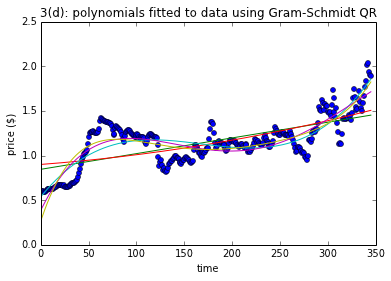
\includegraphics[width=0.5\textwidth]{p3fig1}
\end{figure}

\begin{verbatim}
Using Householder QR factorization:

Degree of fitted polynomial = 1

 P(T) = a*T + b
a = 0.00175825993442
b = 0.845568857432
relative residual = 0.172859206551

Degree of fitted polynomial = 2

 P(T) = a*T^2 + b*T + c
a = 2.72895864077e-06
b = 0.000814040244717
c = 0.900176229486
relative residual = 0.17163894223

Degree of fitted polynomial = 3

 P(T) = a*T^3 + b*T^2 + c*T + d
a = 1.73416859413e-07
b = -8.72743913947e-05
c = 0.013288539243
d = 0.537894744924
relative residual = 0.12834217887

Degree of fitted polynomial = 4

 P(T) = a*T^4 + b*T^3 + c*T^2 + d*T + e
a = -7.20779692429e-10
b = 6.72196406574e-07
c = -0.000198324609702
d = 0.0218559686433
e = 0.387748406167
relative residual = 0.121557884431

Degree of fitted polynomial = 5

 P(T) = a*T^5 + b*T^4 + c*T^3 + d*T^2 + e*T + f
a = 5.9204096951e-12
b = -5.84193407869e-09
c = 2.24838379059e-06
d = -0.000403281743497
e = 0.0320456311369
f = 0.267845555303
relative residual = 0.117970278841
\end{verbatim}

\begin{figure}[H]
  \centering
    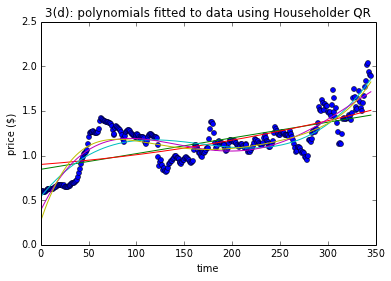
\includegraphics[width=0.5\textwidth]{p3fig2}
\end{figure}

\begin{verbatim}
Using numpy least squares:

Degree of polynomial to fit = 1

 P(T) = a*T + b
a = 0.00175825993442
b = 0.845568857432
relative residual = 0.172859206551

Degree of polynomial to fit = 2

 P(T) = a*T^2 + b*T + c
a = 2.7289586408e-06
b = 0.000814040244717
c = 0.900176229486
relative residual = 0.17163894223

Degree of polynomial to fit = 3

 P(T) = a*T^3 + b*T^2 + c*T + d
a = 1.73416859413e-07
b = -8.72743913947e-05
c = 0.013288539243
d = 0.537894744924
relative residual = 0.12834217887

Degree of polynomial to fit = 4

 P(T) = a*T^4 + b*T^3 + c*T^2 + d*T + e
a = -7.20779692429e-10
b = 6.72196406574e-07
c = -0.000198324609702
d = 0.0218559686433
e = 0.387748406167
relative residual = 0.121557884431

Degree of polynomial to fit = 5

 P(T) = a*T^5 + b*T^4 + c*T^3 + d*T^2 + e*T + f
a = 5.92040969509e-12
b = -5.84193407869e-09
c = 2.24838379058e-06
d = -0.000403281743497
e = 0.0320456311369
f = 0.267845555303
relative residual = 0.117970278841
\end{verbatim}

\begin{figure}[H]
  \centering
    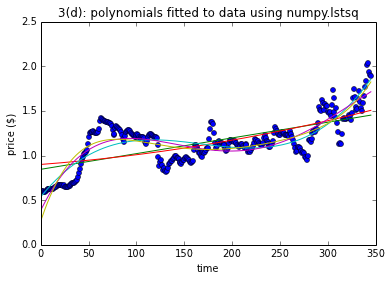
\includegraphics[width=0.5\textwidth]{p3fig3}
\end{figure}

The methods do not seem to differ much. Each method gives approximately the same relative residual $ \| Ax - b \|/\|b\| $. For the $QR$-factorization for the random matrices, the one that uses modified Gram-Schmidt procedure appears to be slightly more accurate.

For the polynomial fits, as the degree of the polynomial increased, the relative residual decreased. However, there was a sharp decrease in the relative residual between $d = 2$ and $d = 3$ and then it doesn't change much. The degree 5 polynomial was the best approximant. This isn't surprising considering it's the one with the largest number of free variables.

\end{enumerate}

\akteachprobhead{%
  Problem 4: Eigenvalue finding
}

\begin{itemize}

\item[(a)] See \verb+cs450hw2p4.py+ for code. Here were my results:

\begin{verbatim}
Part A: inverse iteration for computing eigenvalues and eigenvectors

Running inverse iteration...

Trial 1
Approximate eigenvalue = 2.13307447535
Approximate eigenvector = [-0.49742503  0.8195891   0.28432735]
Number of iterations = 12
Trial 2
Approximate eigenvalue = 2.13307447535
Approximate eigenvector = [-0.49742503  0.8195891   0.28432735]
Number of iterations = 15
Trial 3
Approximate eigenvalue = 2.13307447535
Approximate eigenvector = [-0.49742503  0.8195891   0.28432735]
Number of iterations = 14
Trial 4
Approximate eigenvalue = 2.13307447535
Approximate eigenvector = [-0.49742503  0.8195891   0.28432735]
Number of iterations = 13
Trial 5
Approximate eigenvalue = 2.13307447535
Approximate eigenvector = [-0.49742503  0.8195891   0.28432735]
Number of iterations = 13
Trial 6
Approximate eigenvalue = 2.13307447535
Approximate eigenvector = [-0.49742503  0.8195891   0.28432735]
Number of iterations = 13
Trial 7
Approximate eigenvalue = 2.13307447535
Approximate eigenvector = [-0.49742503  0.8195891   0.28432735]
Number of iterations = 14
Trial 8
Approximate eigenvalue = 2.13307447535
Approximate eigenvector = [-0.49742503  0.8195891   0.28432735]
Number of iterations = 13
Trial 9
Approximate eigenvalue = 2.13307447535
Approximate eigenvector = [-0.49742503  0.8195891   0.28432735]
Number of iterations = 13
Trial 10
Approximate eigenvalue = 2.13307447535
Approximate eigenvector = [-0.49742503  0.8195891   0.28432735]
Number of iterations = 14
\end{verbatim}

\item[(b)] See \verb+cs450hw2p4.py+ for code. Here were my results:

\begin{verbatim}
Part B: Using Rayleigh quotient iteration for computing eigenvalues and eigenvectors

Running Rayleigh Quotient iteration...

Trial 1
Approximate eigenvalue = 2.13307447535
Approximate eigenvector = [-0.49742503  0.8195891   0.28432735]
Number of iterations = 6
Trial 2
Approximate eigenvalue = 0.578933385691
Approximate eigenvector = [-0.0431682  -0.35073145  0.9354806 ]
Number of iterations = 6
Trial 3
Approximate eigenvalue = 7.28799213896
Approximate eigenvector = [ 0.86643225  0.45305757  0.20984279]
Number of iterations = 6
Trial 4
Approximate eigenvalue = 2.13307447535
Approximate eigenvector = [-0.49742503  0.8195891   0.28432735]
Number of iterations = 5
Trial 5
Approximate eigenvalue = 7.28799213896
Approximate eigenvector = [ 0.86643225  0.45305757  0.20984279]
Number of iterations = 4
Trial 6
Approximate eigenvalue = 7.28799213896
Approximate eigenvector = [ 0.86643225  0.45305757  0.20984279]
Number of iterations = 5
Trial 7
Approximate eigenvalue = 7.28799213896
Approximate eigenvector = [ 0.86643225  0.45305757  0.20984279]
Number of iterations = 5
Trial 8
Approximate eigenvalue = 2.13307447535
Approximate eigenvector = [-0.49742503  0.8195891   0.28432735]
Number of iterations = 5
Trial 9
Approximate eigenvalue = 7.28799213896
Approximate eigenvector = [ 0.86643225  0.45305757  0.20984279]
Number of iterations = 6
Trial 10
Approximate eigenvalue = 7.28799213896
Approximate eigenvector = [ 0.86643225  0.45305757  0.20984279]
Number of iterations = 5
\end{verbatim}

\item[(c)] For inverse iteration, it always seemed to converge to the same eigenvalue. For Rayleigh quotient iteration, the eigenvalue converged to depended on the starting vector. Rayleigh quotient iteration also was faster, stopping after around half the steps that it took inverse iteration.

\item[(d)] See \verb+cs450hw2p4.py+ for code. Here were my results:

\begin{verbatim}
Comparing iterative methods to actual eigenvectors and eigenvalues

Using inverse iteration:

Trial 1
Starting vector: [ 0.15416284  0.7400497   0.26331502]
Number of iterations: 12

Approximate eigenvalue: 2.13307447535
Actual eigenvalue: (2.13307447535+0j)
Relative Error in eigenvalue: 0.0

Approximate eigenvector: [-0.49742503  0.8195891   0.28432735]
Actual eigenvector: [-0.45305757  0.8195891   0.35073145]
Relative Error in eigenvector: 0.0798622270523

Trial 2
Starting vector: [ 0.53373939  0.01457496  0.91874701]
Number of iterations: 15

Approximate eigenvalue: 2.13307447535
Actual eigenvalue: (2.13307447535+0j)
Relative Error in eigenvalue: 2.08192079078e-16

Approximate eigenvector: [-0.49742503  0.8195891   0.28432735]
Actual eigenvector: [-0.45305757  0.8195891   0.35073145]
Relative Error in eigenvector: 0.0798622270524

Trial 3
Starting vector: [ 0.90071485  0.03342143  0.95694934]
Number of iterations: 14

Approximate eigenvalue: 2.13307447535
Actual eigenvalue: (2.13307447535+0j)
Relative Error in eigenvalue: 6.24576237233e-16

Approximate eigenvector: [-0.49742503  0.8195891   0.28432735]
Actual eigenvector: [-0.45305757  0.8195891   0.35073145]
Relative Error in eigenvector: 0.0798622270523

Trial 4
Starting vector: [ 0.13720932  0.28382835  0.60608318]
Number of iterations: 13

Approximate eigenvalue: 2.13307447535
Actual eigenvalue: (2.13307447535+0j)
Relative Error in eigenvalue: 2.08192079078e-16

Approximate eigenvector: [-0.49742503  0.8195891   0.28432735]
Actual eigenvector: [-0.45305757  0.8195891   0.35073145]
Relative Error in eigenvector: 0.0798622270524

Trial 5
Starting vector: [ 0.94422514  0.85273554  0.00225923]
Number of iterations: 13

Approximate eigenvalue: 2.13307447535
Actual eigenvalue: (2.13307447535+0j)
Relative Error in eigenvalue: 2.08192079078e-16

Approximate eigenvector: [-0.49742503  0.8195891   0.28432735]
Actual eigenvector: [-0.45305757  0.8195891   0.35073145]
Relative Error in eigenvector: 0.0798622270523

Trial 6
Starting vector: [ 0.52122603  0.55203763  0.48537741]
Number of iterations: 13

Approximate eigenvalue: 2.13307447535
Actual eigenvalue: (2.13307447535+0j)
Relative Error in eigenvalue: 4.16384158155e-16

Approximate eigenvector: [-0.49742503  0.8195891   0.28432735]
Actual eigenvector: [-0.45305757  0.8195891   0.35073145]
Relative Error in eigenvector: 0.0798622270524

Trial 7
Starting vector: [ 0.76813415  0.16071675  0.76456045]
Number of iterations: 14

Approximate eigenvalue: 2.13307447535
Actual eigenvalue: (2.13307447535+0j)
Relative Error in eigenvalue: 4.16384158155e-16

Approximate eigenvector: [-0.49742503  0.8195891   0.28432735]
Actual eigenvector: [-0.45305757  0.8195891   0.35073145]
Relative Error in eigenvector: 0.0798622270524

Trial 8
Starting vector: [ 0.0208098   0.13521018  0.11627302]
Number of iterations: 13

Approximate eigenvalue: 2.13307447535
Actual eigenvalue: (2.13307447535+0j)
Relative Error in eigenvalue: 2.08192079078e-16

Approximate eigenvector: [-0.49742503  0.8195891   0.28432735]
Actual eigenvector: [-0.45305757  0.8195891   0.35073145]
Relative Error in eigenvector: 0.0798622270523

Trial 9
Starting vector: [ 0.30989758  0.67145265  0.47122978]
Number of iterations: 13

Approximate eigenvalue: 2.13307447535
Actual eigenvalue: (2.13307447535+0j)
Relative Error in eigenvalue: 4.16384158155e-16

Approximate eigenvector: [-0.49742503  0.8195891   0.28432735]
Actual eigenvector: [-0.45305757  0.8195891   0.35073145]
Relative Error in eigenvector: 0.0798622270523

Trial 10
Starting vector: [ 0.8161683   0.28958678  0.73312598]
Number of iterations: 14

Approximate eigenvalue: 2.13307447535
Actual eigenvalue: (2.13307447535+0j)
Relative Error in eigenvalue: 6.24576237233e-16

Approximate eigenvector: [-0.49742503  0.8195891   0.28432735]
Actual eigenvector: [-0.45305757  0.8195891   0.35073145]
Relative Error in eigenvector: 0.0798622270523


Using Rayleigh quotient iteration:

Trial 1
Starting vector: [ 0.15416284  0.7400497   0.26331502]
Number of iterations: 6

Approximate eigenvalue: 2.13307447535
Actual eigenvalue: (2.13307447535+0j)
Relative Error in eigenvalue: 6.24576237233e-16

Approximate eigenvector: [-0.49742503  0.8195891   0.28432735]
Actual eigenvector: [-0.45305757  0.8195891   0.35073145]
Relative Error in eigenvector: 0.0798622270523

Trial 2
Starting vector: [ 0.53373939  0.01457496  0.91874701]
Number of iterations: 6

Approximate eigenvalue: 0.578933385691
Actual eigenvalue: (0.578933385691+0j)
Relative Error in eigenvalue: 0.0

Approximate eigenvector: [-0.0431682  -0.35073145  0.9354806 ]
Actual eigenvector: [ 0.20984279 -0.28432735  0.9354806 ]
Relative Error in eigenvector: 0.26157994371

Trial 3
Starting vector: [ 0.90071485  0.03342143  0.95694934]
Number of iterations: 6

Approximate eigenvalue: 7.28799213896
Actual eigenvalue: (7.28799213896+0j)
Relative Error in eigenvalue: 8.53081180572e-16

Approximate eigenvector: [ 0.86643225  0.45305757  0.20984279]
Actual eigenvector: [ 0.86643225  0.49742503 -0.0431682 ]
Relative Error in eigenvector: 0.256871632202

Trial 4
Starting vector: [ 0.13720932  0.28382835  0.60608318]
Number of iterations: 5

Approximate eigenvalue: 2.13307447535
Actual eigenvalue: (2.13307447535+0j)
Relative Error in eigenvalue: 6.24576237233e-16

Approximate eigenvector: [-0.49742503  0.8195891   0.28432735]
Actual eigenvector: [-0.45305757  0.8195891   0.35073145]
Relative Error in eigenvector: 0.0798622270523

Trial 5
Starting vector: [ 0.94422514  0.85273554  0.00225923]
Number of iterations: 4

Approximate eigenvalue: 7.28799213896
Actual eigenvalue: (7.28799213896+0j)
Relative Error in eigenvalue: 8.53081180572e-16

Approximate eigenvector: [ 0.86643225  0.45305757  0.20984279]
Actual eigenvector: [ 0.86643225  0.49742503 -0.0431682 ]
Relative Error in eigenvector: 0.256871632202

Trial 6
Starting vector: [ 0.52122603  0.55203763  0.48537741]
Number of iterations: 5

Approximate eigenvalue: 7.28799213896
Actual eigenvalue: (7.28799213896+0j)
Relative Error in eigenvalue: 8.53081180572e-16

Approximate eigenvector: [ 0.86643225  0.45305757  0.20984279]
Actual eigenvector: [ 0.86643225  0.49742503 -0.0431682 ]
Relative Error in eigenvector: 0.256871632202

Trial 7
Starting vector: [ 0.76813415  0.16071675  0.76456045]
Number of iterations: 5

Approximate eigenvalue: 7.28799213896
Actual eigenvalue: (7.28799213896+0j)
Relative Error in eigenvalue: 8.53081180572e-16

Approximate eigenvector: [ 0.86643225  0.45305757  0.20984279]
Actual eigenvector: [ 0.86643225  0.49742503 -0.0431682 ]
Relative Error in eigenvector: 0.256871632202

Trial 8
Starting vector: [ 0.0208098   0.13521018  0.11627302]
Number of iterations: 5

Approximate eigenvalue: 2.13307447535
Actual eigenvalue: (2.13307447535+0j)
Relative Error in eigenvalue: 2.08192079078e-16

Approximate eigenvector: [-0.49742503  0.8195891   0.28432735]
Actual eigenvector: [-0.45305757  0.8195891   0.35073145]
Relative Error in eigenvector: 0.0798622270523

Trial 9
Starting vector: [ 0.30989758  0.67145265  0.47122978]
Number of iterations: 6

Approximate eigenvalue: 7.28799213896
Actual eigenvalue: (7.28799213896+0j)
Relative Error in eigenvalue: 6.09343700408e-16

Approximate eigenvector: [ 0.86643225  0.45305757  0.20984279]
Actual eigenvector: [ 0.86643225  0.49742503 -0.0431682 ]
Relative Error in eigenvector: 0.256871632202

Trial 10
Starting vector: [ 0.8161683   0.28958678  0.73312598]
Number of iterations: 5

Approximate eigenvalue: 7.28799213896
Actual eigenvalue: (7.28799213896+0j)
Relative Error in eigenvalue: 8.53081180572e-16

Approximate eigenvector: [ 0.86643225  0.45305757  0.20984279]
Actual eigenvector: [ 0.86643225  0.49742503 -0.0431682 ]
Relative Error in eigenvector: 0.256871632202
\end{verbatim}

\item[(e)] See \verb+cs450hw2p4.py+ for code. The Rayleigh quotient iteration converged more rapidly with approximately the same error in the results. Here were my results:

\begin{verbatim}
Starting vector: [1 4 2]

Using inverse iteration:

Number of iterations: 12

Approximate eigenvalue: 2.13307447535
Actual eigenvalue: (2.13307447535+0j)
Relative Error in eigenvalue: 4.16384158155e-16

Approximate eigenvector: [-0.49742503  0.8195891   0.28432735]
Actual eigenvector: [-0.45305757  0.8195891   0.35073145]
Relative Error in eigenvector: 0.0798622270523


Using Rayleigh quotient iteration:

Number of iterations: 7

Approximate eigenvalue: 2.13307447535
Actual eigenvalue: (2.13307447535+0j)
Relative Error in eigenvalue: 6.24576237233e-16

Approximate eigenvector: [-0.49742503  0.8195891   0.28432735]
Actual eigenvector: [-0.45305757  0.8195891   0.35073145]
Relative Error in eigenvector: 0.0798622270523
\end{verbatim}



\end{itemize}

\akteachprobhead{%
  Problem 5:
}

\begin{enumerate}

\item[(a)] See \verb+cs450hw2p5.py+ for code. Here were my results:

\begin{figure}[H]
  \centering
    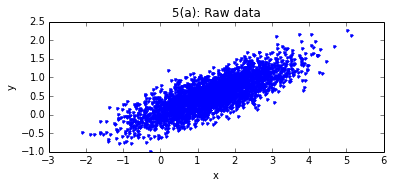
\includegraphics[width=0.5\textwidth]{p5fig1}
\end{figure}

\item[(b)] See \verb+cs450hw2p5.py+ for code. Here were my results:

\begin{figure}[H]
  \centering
    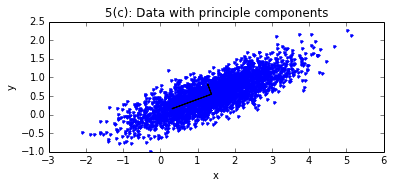
\includegraphics[width=0.5\textwidth]{p5fig2}
\end{figure}

\item[(c)] See \verb+cs450hw2p5.py+ for code. Here were my results:

\begin{verbatim}
Relative error between Y and U*Sigma*V.T = 2.77844520271e-16
\end{verbatim}

\item[(d)] See \verb+cs450hw2p5.py+ for code. Here were my results:

\begin{figure}[H]
  \centering
    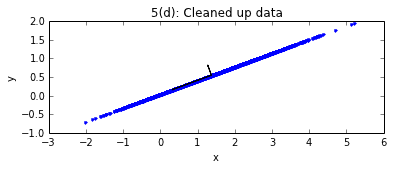
\includegraphics[width=0.5\textwidth]{p5fig3}
\end{figure}

We've cleaned the data up in the direction of the smaller principle component, eliminating noise. This cuts the size of the data stored in half.

\end{enumerate}

\end{document}
